\documentclass[12pt, twoside]{article}
\usepackage[letterpaper, margin=1in, head=30pt, headsep=0.1in]{geometry}
\usepackage[english]{babel}
\usepackage[utf8]{inputenc}
\usepackage{amsmath}
\usepackage{amsfonts}
\usepackage{amssymb}
\usepackage{tikz}
\usetikzlibrary{quotes, angles}

\usepackage{graphicx}
\usepackage{enumitem}
\usepackage{multicol}

%\usepackage{pgfplots}
%\pgfplotsset{width=10cm,compat=1.9}
%\usepgfplotslibrary{statistics}
%\usepackage{pgfplotstable}
%\usepackage{tkz-fct}
%\usepackage{venndiagram}

\usepackage{fancyhdr}
\pagestyle{fancy}
\fancyhf{}
\renewcommand{\headrulewidth}{0pt} % disable the underline of the header
\raggedbottom
\newif\ifmeta
\metatrue %print standards and topics tags

\title{Math AI Worksheet Generator and Formative Assessment System}
\author{Chris Huson}
\date{January 2021}

%\fancyhead[RE]{\thepage}
%\fancyhead[RO]{\thepage \\ Name: \hspace{3cm}}
%\fancyhead[L]{BECA / Dr. Huson / 10th Grade Geometry\\* 7 June 2019}
%
%\begin{document}
%\subsubsection*{13.7 Homework: Cross sections, distance applications}
%\fancyhead[L]{BECA / Dr. Huson / Geometry 03-Volume+angle-bisectors\\* pset ID: 34}

\begin{document}

\subsubsection*{5.12 Skills ReQuiz: Area and volume situations}
\begin{enumerate}

\item Find the area of rectangle $ABCD$ having length $l=10$ and width $w=3 \frac{3}{4}$. Start with a formula of this form, substituting the given values: \\[0.5cm]
$A = l \times w$
  \begin{flushright}
  \begin{tikzpicture}[scale=1.25]
    \draw [-, thick] (0,0)--(4.5,0)--(4.5,2)--(0,2)--cycle;
    \draw [fill] (0,0) circle [radius=0.05] node[left]{$A$};
    \draw [fill] (4.5,0) circle [radius=0.05] node[right]{$B$};
    \draw [fill] (4.5,2) circle [radius=0.05] node[right]{$C$};
    \draw [fill] (0,2) circle [radius=0.05] node[left]{$D$};
    \node at (5, 1){$3 \frac{3}{4}$};
    \node at (2.25, -0.5){$10$};
    %\node at (2.25, 1){$A = 15$};
  \end{tikzpicture}
  \end{flushright}

\newpage
\item Find the volume of a rectangular prism (box). Its length is $l=22$ inches, its height $h=12$ inches, and depth is $w=9$ inches. Start with the equation \\[0.5cm]
$V = l \times w \times h$
  \begin{flushright}
    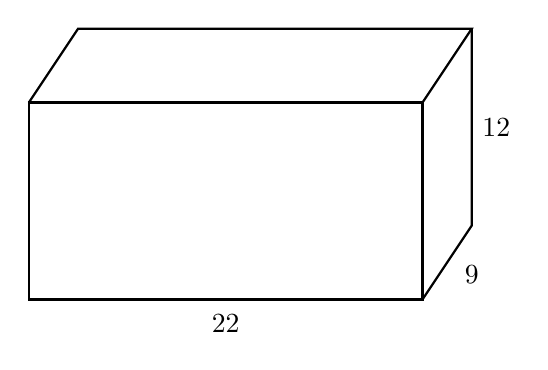
\begin{tikzpicture}[scale=1.25]
      \draw [-, thick] (0,0)--(4,0)--(4,2)--(0,2)--cycle;
      \draw [-, thick] (0,2)--(0.5,2.75)--(4.5,2.75)--(4,2);
      \draw [-, thick] (4,0)--(4.5,0.75)--(4.5,2.75);
      \node at (4.75, 1.75){$12$};
      \node at (2, -0.25){$22$};
      \node at (4.5, 0.25){$9$};
    \end{tikzpicture}
  \end{flushright}
  
\newpage
\item A parallelogram is shown on the $x$-$y$ plane having a base $b=4.25$ and height $h=7.0$. 
  \begin{multicols}{2}
    Find its area, showing the calculation.
      \begin{flushright}
      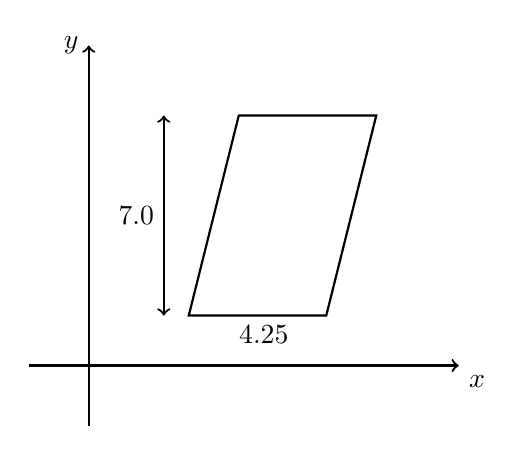
\begin{tikzpicture}[scale=.635]
        %\draw [help lines] (-1,-1) grid (9,6);
        \draw [thick, ->] (-1.2,0) -- (7.4,0) node [below right] {$x$};
        \draw [thick, ->] (0,-1.2)--(0,6.4) node [left] {$y$};
        \draw [<->, thick] (1.5,1)--(1.5,5);
        \draw [-, thick] (2,1)--(4.75,1)--(5.75,5)--(3,5)--cycle;
        \node at (3.5,1)[below]{$4.25$};
        \node at (1.5,3)[left]{$7.0$};
      \end{tikzpicture}
      \end{flushright}
  \end{multicols} 

\newpage
\item The $\triangle ABC$ is shown below with $A(3,1)$, $B(7,1)$, and $C(2,6)$. The length of the base of the triangle is $AB=4$.
  \begin{multicols}{2}
    \begin{enumerate}
      \item Find the height $h$.
      \item Find the triangle's area, showing the calculation. \vspace{2cm}
      \end{enumerate}
      \begin{flushright}
      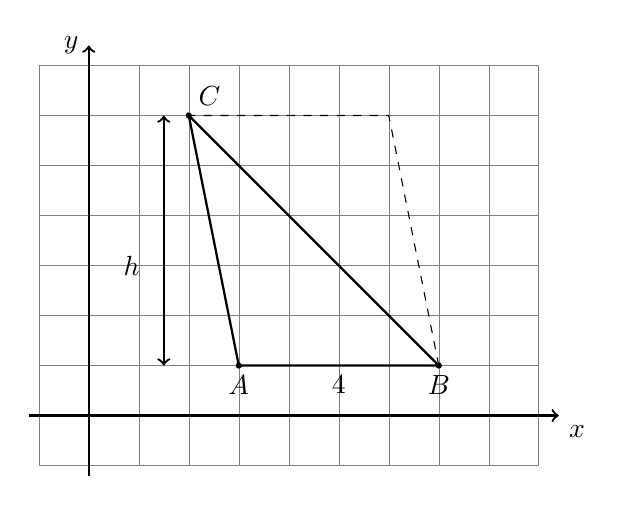
\begin{tikzpicture}[scale=.635]
        \draw [help lines] (-1,-1) grid (9,7);
        \draw [thick, ->] (-1.2,0) -- (9.4,0) node [below right] {$x$};
        \draw [thick, ->] (0,-1.2)--(0,7.4) node [left] {$y$};
        \draw [<->, thick] (1.5,1)--(1.5,6);
        \draw [-, thick] (3,1)--(7,1)--(2,6)--cycle;
        \draw [-, dashed] (7,1)--(6,6)--(2,6);
        \draw [fill] (3,1) circle [radius=0.05] node[below] {$A$};
        \draw [fill] (7,1) circle [radius=0.05] node[below] {$B$};
        \draw [fill] (2,6) circle [radius=0.05] node[above right] {$C$};
        \node at (5,1)[below]{$4$};
        \node at (0.5,3)[right]{$h$};
      \end{tikzpicture}
      \end{flushright}
  \end{multicols} 

\newpage
\item Find the width of the base of a rectangle with area $A=75$ and height $h=15$. Start with the form (use $b$ or $x$): \\[0.5cm]
$A = b \times h = 75$
  \begin{flushright}
  \begin{tikzpicture}[scale=1.25]
    \draw [-, thick] (0,0)--(2,0)--(2,6)--(0,6)--cycle;
    \node at (2.5, 3){$15$};
    \node at (1, -0.5){$?$};
    \node at (1, 3){$75$};
  \end{tikzpicture}
  \end{flushright}

\newpage
\item Find the height of the $\triangle BLM$, having an area of $A=42$ and base $BL=7$.
  \begin{multicols}{2}
    Start by substituting values in the area formula: \\[0.5cm]
    $\displaystyle A = \frac{1}{2} bh = 42$ \vspace{2cm}
      \begin{flushright}
      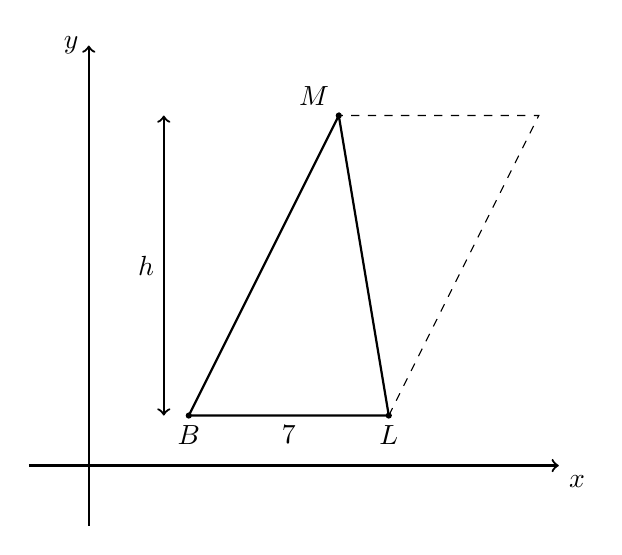
\begin{tikzpicture}[scale=.635]
        %\draw [help lines] (-1,-1) grid (9,6);
        \draw [thick, ->] (-1.2,0) -- (9.4,0) node [below right] {$x$};
        \draw [thick, ->] (0,-1.2)--(0,8.4) node [left] {$y$};
        \draw [<->, thick] (1.5,1)--(1.5,7);
        \draw [-, thick] (2,1)--(6,1)--(5,7)--cycle;
        \draw [-, dashed] (6,1)--(9,7)--(5,7);
        \draw [fill] (2,1) circle [radius=0.05] node[below] {$B$};
        \draw [fill] (6,1) circle [radius=0.05] node[below] {$L$};
        \draw [fill] (5,7) circle [radius=0.05] node[above left] {$M$};
        \node at (4,1)[below]{$7$};
        \node at (1.5,4)[left]{$h$};
      \end{tikzpicture}
      \end{flushright}
  \end{multicols}

\newpage
\item The rectangular prism shown has a volume of $V=1815$ cubic centimeters. Its base measures $l=12.5$ cm by $w=8.8$ cm. \\[0.5cm]
Find its height in centimeters. Begin by writing the following formula with values substituted: \\[0.5cm]
$V = l \times w \times h = 1815$
\begin{flushright}
  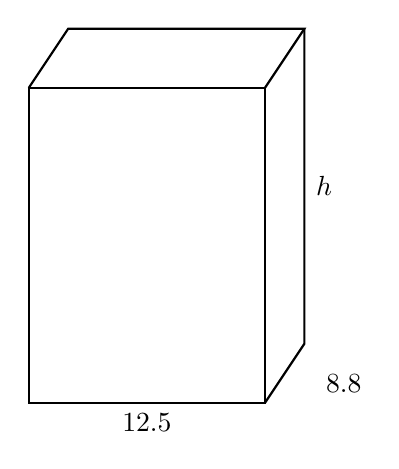
\begin{tikzpicture}[scale=1]
    \draw [-, thick] (0,0)--(3,0)--(3,4)--(0,4)--cycle;
    \draw [-, thick] (0,4)--(0.5,4.75)--(3.5,4.75)--(3,4);
    \draw [-, thick] (3,0)--(3.5,0.75)--(3.5,4.75);
    \node at (3.75, 2.75){$h$};
    \node at (1.5, -0.25){$12.5$};
    \node at (4, 0.25){$8.8$};
  \end{tikzpicture}
\end{flushright}

\newpage
\item Find the length of the base of a triangle with area $A=30$ and height $h=6 \frac{2}{3}$. Start with the form (use $b$ or $x$): \\[0.5cm]
$A = \frac{1}{2} \times b \times h = 30$
  \begin{flushright}
  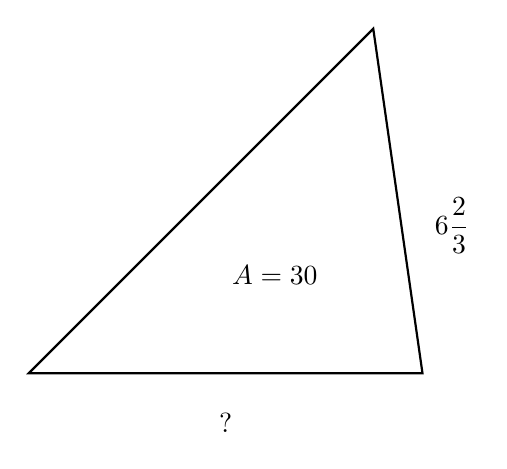
\begin{tikzpicture}[scale=1.25]
    \draw [-, thick] (-1,0)--(3,0)--(2.5,3.5)--cycle;
    \node at (3.3, 1.5){$\displaystyle 6 \frac{2}{3}$};
    \node at (1, -0.5){$?$};
    \node at (1.5, 1){$A = 30$};
  \end{tikzpicture}
  \end{flushright}

\newpage
\item Find the area of the $\triangle ABC$, shown below, with $A(1,2)$, $B(7,4)$, and $C(4,8)$. 
  \begin{multicols}{2}
    Hint: Subtract the areas of the three right triangles from the area of the red square.
      \begin{flushright}
      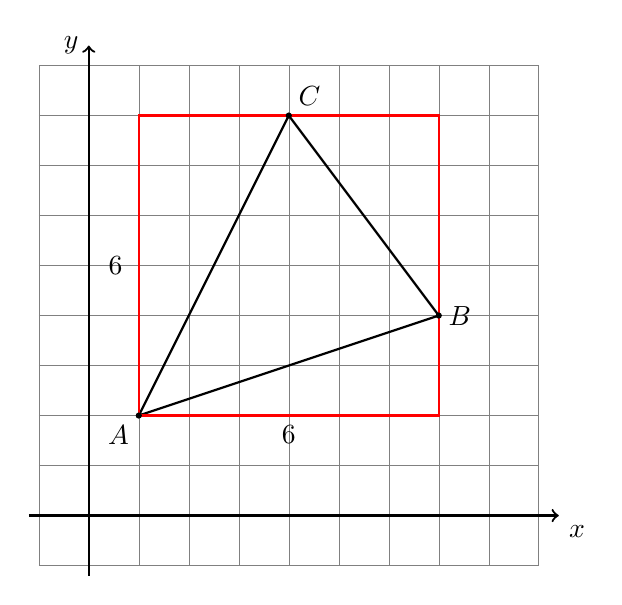
\begin{tikzpicture}[scale=.635]
        \draw [help lines] (-1,-1) grid (9,9);
        \draw [thick, ->] (-1.2,0) -- (9.4,0) node [below right] {$x$};
        \draw [thick, ->] (0,-1.2)--(0,9.4) node [left] {$y$};
        %\draw [<->, thick] (0.5,1)--(0.5,5);
        \draw [-, thick] (1,2)--(7,4)--(4,8)--cycle;
        \draw [-, thick, red] (1,2)--(7,2)--(7,8)--(1,8)--cycle;
        \draw [fill] (1,2) circle [radius=0.05] node[below left] {$A$};
        \draw [fill] (7,4) circle [radius=0.05] node[right] {$B$};
        \draw [fill] (4,8) circle [radius=0.05] node[above right] {$C$};
        \node at (4,2)[below]{$6$};
        \node at (0.2,5)[right]{$6$};
      \end{tikzpicture}
      \end{flushright}
  \end{multicols} 

\newpage
\item A rectangular prism has a square base. Its volume is $V=162$ cubic centimeters and its height is $h=8$ cm.
  \begin{multicols}{2}
    Calculate the dimensions of its base.
    \begin{flushright}
      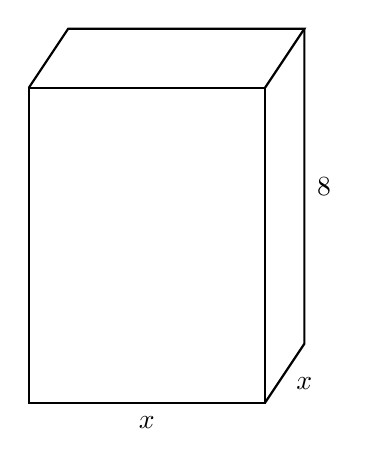
\begin{tikzpicture}[scale=1]
        \draw [-, thick] (0,0)--(3,0)--(3,4)--(0,4)--cycle;
        \draw [-, thick] (0,4)--(0.5,4.75)--(3.5,4.75)--(3,4);
        \draw [-, thick] (3,0)--(3.5,0.75)--(3.5,4.75);
        \node at (3.75, 2.75){$8$};
        \node at (1.5, -0.25){$x$};
        \node at (3.5, 0.25){$x$};
      \end{tikzpicture}
    \end{flushright}
  \end{multicols}


\end{enumerate}
\end{document}